\section{Introduction}
\begin{figure}[!t]
    \centering
    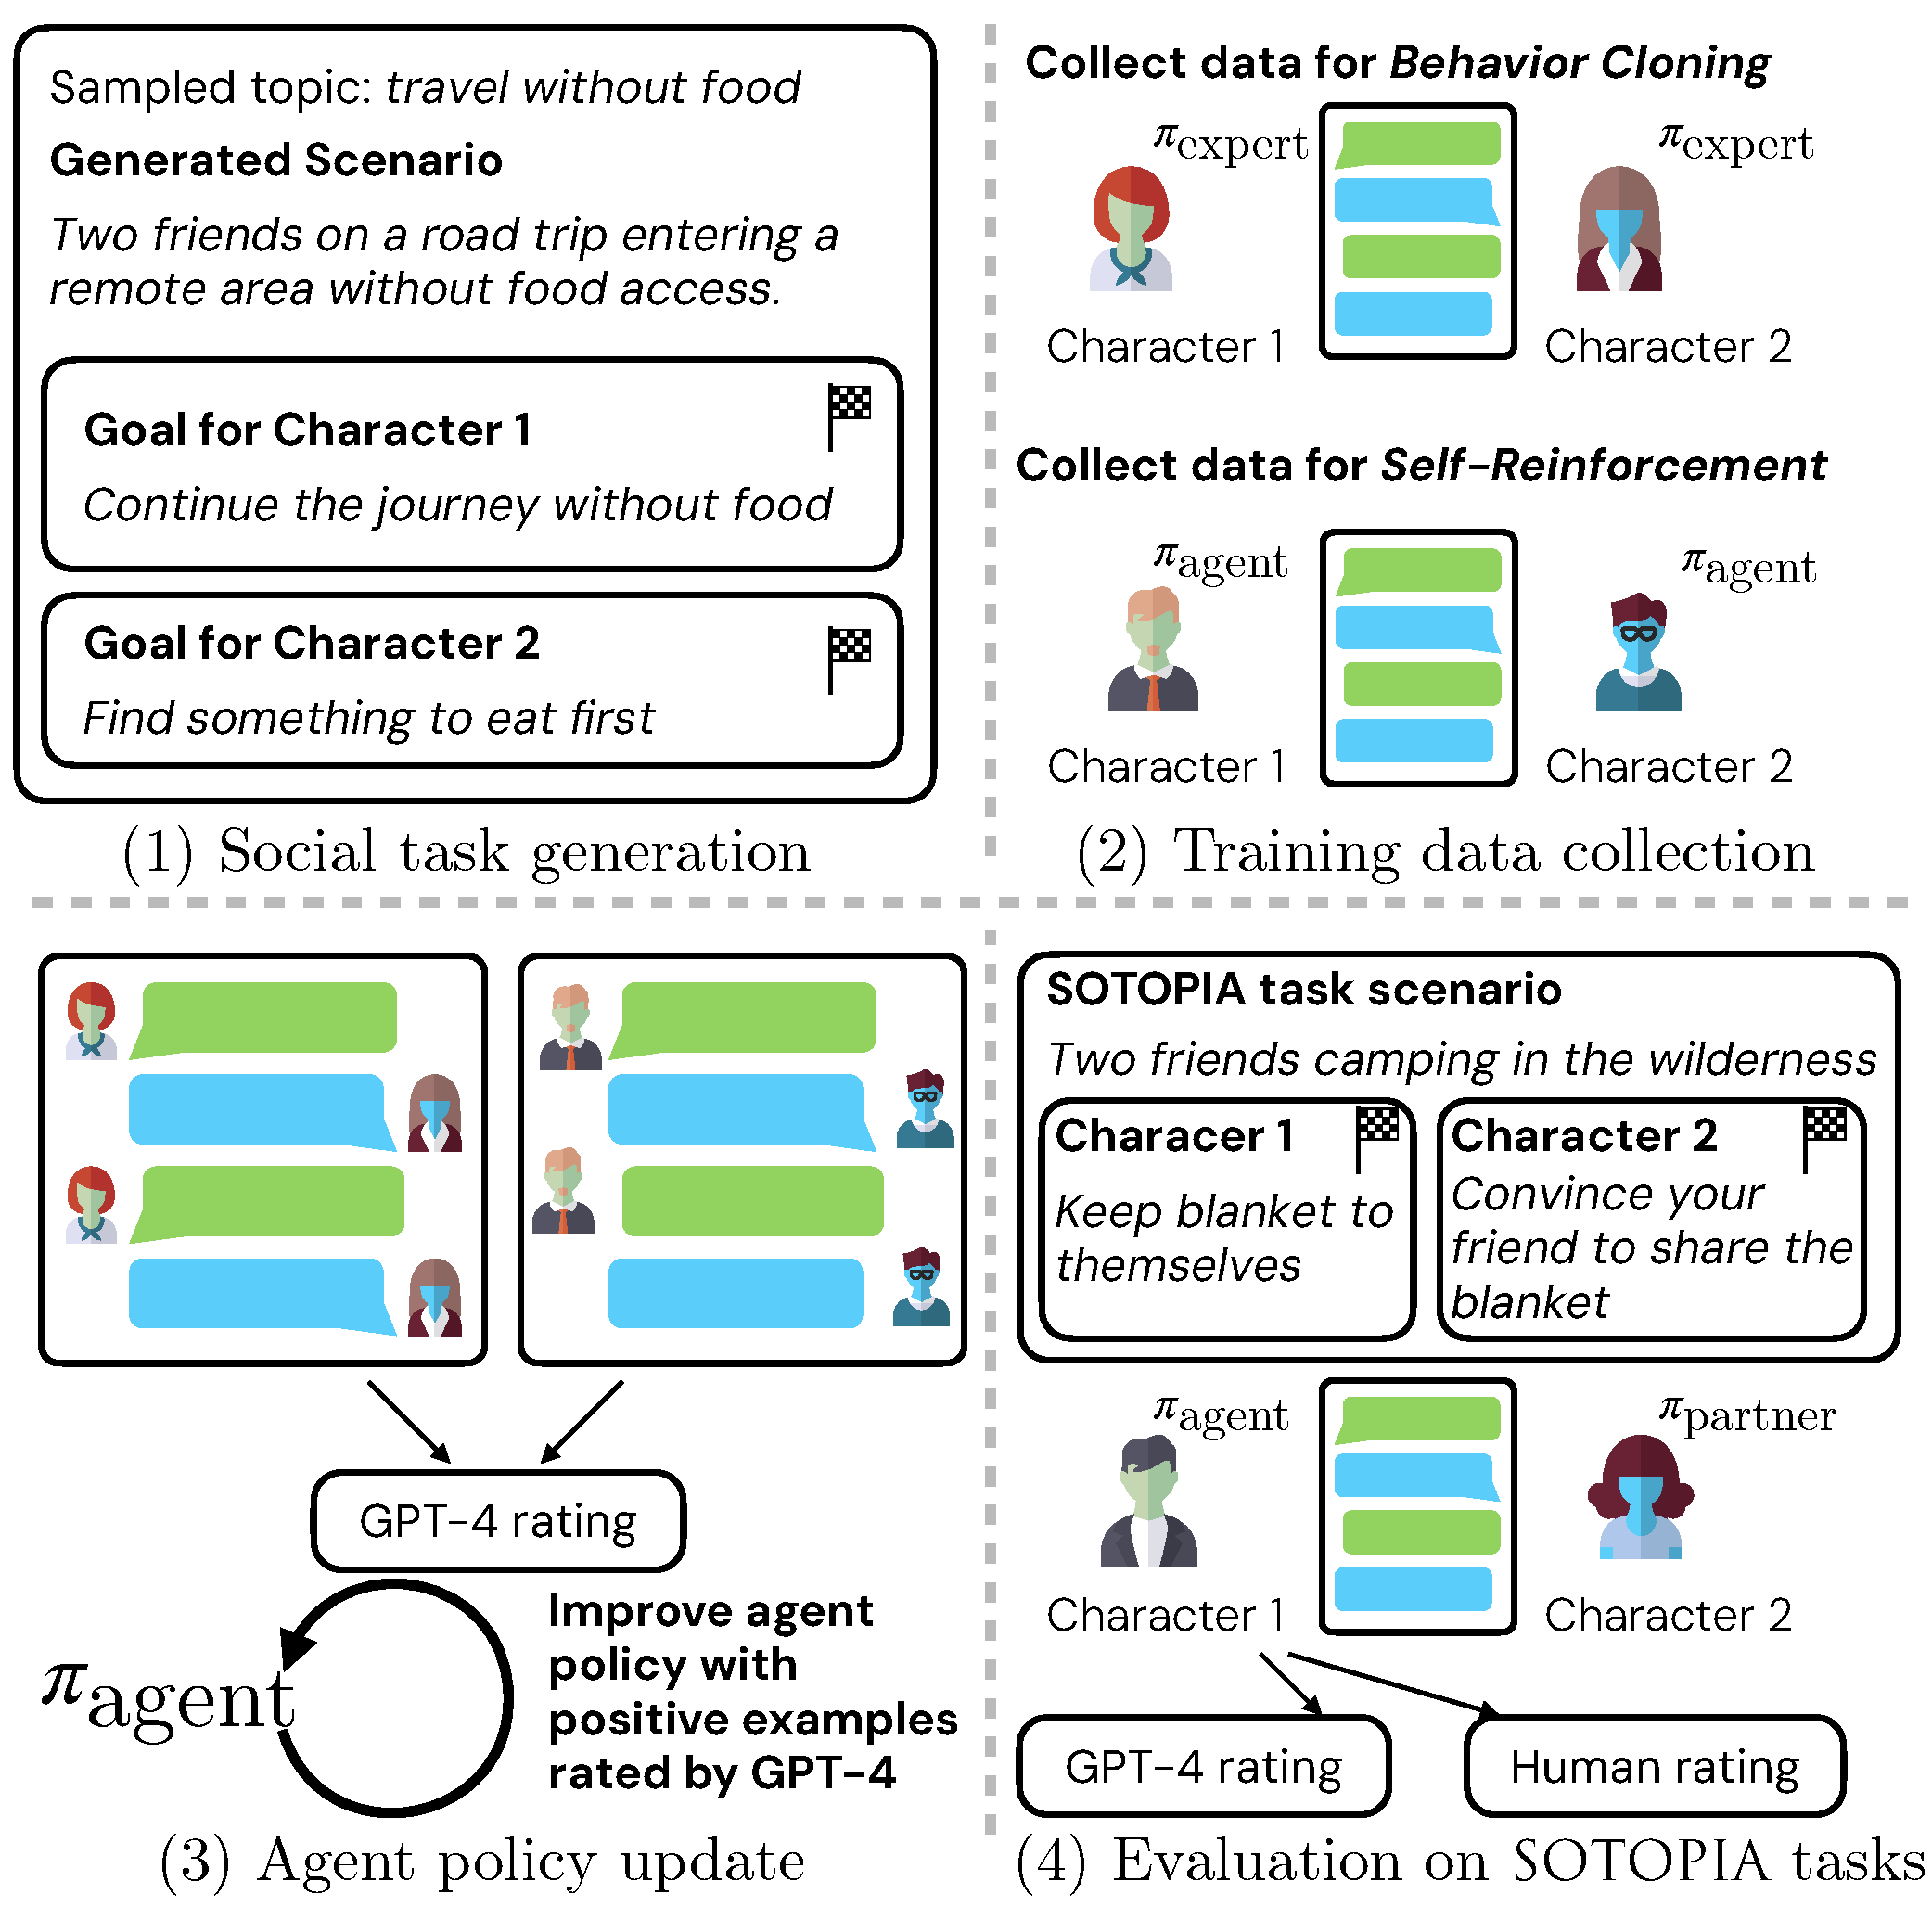
\includegraphics[width=\linewidth]{figs/acl2024_teaser.pdf}
    \caption{We propose \model, which (1) automatically generates new social tasks, (2) collects data from both expert policy and agent policy for training, and (3) updates agent policy based on positive data rated by GPT-4. We implement (4) human and GPT-4 evaluation on our trained agent performing tasks in \sotopia with the partner agent. Our training paradigms include behavior cloning and self-reinforcement. For evaluation, we use  \sotopiaeval and a fixed partner policy (GPT-3.5-based). Note that the character profiles are omitted and the examples are shortened for demonstration.}
    \label{fig:pipeline}
    \vspace{-15pt}
\end{figure}

Machine social intelligence is crucial to productive human-machine interaction~\cite{gweon2023socially}. For instance, to achieve real-time social interactions with users, virtual agents should not only emulate human verbal and non-verbal social behaviors but also manage social skills such as cooperation and negotiation. 
However, the social intelligence of large language models (LLMs) 
still lags behind humans in various aspects, including theory-of-mind \citep{sap2023neural,ullman2023large, shapira2023clever}, following social norms \citep{weidinger2021ethical}, and navigating diverse goal-driven social scenarios~\citep{sotopia}. This underscores the challenge to bridge the gap and empower LLM agents to navigate social situations with human-like social decision-making abilities and values. 

Inspired by the way that humans acquire these social abilities through exploration, interaction, and self-reinforcement~\citep{Tomasello2021becoming, inferential-social-learning}, 
we propose an \emph{interactive learning} method, \model (Figure~\ref{fig:pipeline}), which improves the social intelligence of language agents through social interactions (e.g., \textsl{the conversation between a seller and a buyer on Craigslist}). 

In \model, we use GPT-4~\cite{openai2023gpt4} to automatically synthesize new social tasks to learn transferable social strategies, similar to open-ended learning~\citep{team2021open} (\hyperref[sec:method_social_task_generation]{Step 1}). 
To simulate the social interaction within a diverse set of agents, we collect interaction data between the agents and an expert policy (GPT-4-based) or between two instances of the agent policy that role-play two sampled characters (\hyperref[sec:method_collecting_social_interaction_data]{Step 2}). To reinforce the positive examples in social interaction, we use GPT-4 to provide ratings of how well the agent is able to achieve its goals and filter the interaction data based on a threshold for this score. Then we update the agent policy with either or both of two paradigms: \emph{behavior cloning} (learning from behaviors of an expert model with strong social skills) and \emph{self-reinforcement} (learning from highly-rated behaviors of the model itself) (\hyperref[sec:agent_policy_update]{Step 3}). We evaluate our method with human and GPT-4-based evaluation on the trained agent models in the \sotopia~\citep{sotopia} environment (\S\ref{subsec:sotopia_environment}).

The closest to our work is Stable Alignment \citep{liu2023training}, which studies social alignment in single-turn question-answering tasks. In contrast, \model improves multi-turn interaction capability under realistic social scenarios beyond verbal communication. \S\ref{sec:safety-section} shows that our method, despite not explicitly designed for improving alignment, trains models to behave more safely and generate fewer toxic responses. 
% distinguishing methodology
Without requiring human involvement and an online reward model~\citep{ziegler2020finetuning, ouyang2022training}, our method is efficient and scalable because it (1) gathers offline social interaction data with LLMs and (2) enables language agents to explore and reinforce the social knowledge of itself and expert models.

Using our method to train socially intelligent agents, we examine the effectiveness of the two training paradigms as well as possible side effects (e.g., loss of knowledge or safety). In addition, by evaluating the social intelligence of our trained models through human judgment, we aim to understand the effectiveness of training LLMs from LLM ratings. Therefore, we propose to answer the following research questions:

\begin{description}

\item[RQ1] Can \model improve the social goal completion ability and the overall social intelligence of language agents?

\item[RQ2] Is LLM rating an effective proxy to human rating for training social intelligence in language agents?

\item[RQ3] How does training with \model influence other capabilities of language agents?

\end{description}

For \textbf{RQ1}, our findings reveal that self-reinforcement notably improves the social goal completion ability of a base 7B LLM as well as one trained with behavior cloning. The best model (trained with behavior cloning followed by self-reinforcement) approaches the performance of GPT-4 according to GPT-4-based evaluation. Regarding \textbf{RQ2}, we observe an increasing gap between GPT-4-based and human evaluation, highlighting the limitations of relying solely on GPT-4-based evaluation for optimizing or evaluating language models. This signals the need for future work on developing alternative evaluator models that can robustly evaluate social interaction. In response to \textbf{RQ3}, our safety evaluation shows that \model improves safety and reduces the toxicity of language models in social tasks. Furthermore, when assessed on the Massive Multitask Language Understanding (MMLU) benchmark~\cite{hendrycks2020measuring}, we demonstrate that \model preserves the original question-answering ability of the models. 
